\section{Plant-wide control}


\subsection{Plant-wide control philosophy and survey table}%0.25 page

Nitroma aimed at developing an effective plant-wide control structure for the entire chemical plant following a general heuristic procedure proposed by \textcite{}. A plant-wide control approach offers many advantages over an individual unit based approach. Firstly, disturbance propagation introduced by multiple recycle loops in the process can be efficiently mitigated. Secondly, the likelihood of conflicts between control loops is reduced, so highly oscillatory behaviour of any control parameter becomes very unlikely. 

The control objectives and consequences associated with poor control were identified during a plant-wide control survey conducted on all major process units. For each potential control loop, a controlled variable and a manipulated variable were identified. The type of sensor and actuator was then selected. All possible disturbances affecting the controlled variable were then listed out. Finally the survey addressed major maintenance issues for each of the process units and proposed solutions to mitigate those issues. The plant wide survey can be found in the Supporting Documentation \Cref{sec:PWS}.


\subsection{Key controls}%stephen

\subsubsection{Throughput and quality control}
Throughput control is an essential part of Nitroma's control strategy as it ensures that the production capacity of the three products can be consistently met. 

A general framework for choosing a suitable throughput manipulator (TPM) has been laid out by \textcite{}. They recommend choosing a valve that directly impacts the reaction rate in the primary reactor of the process while having minimal impact on the separation system. In principle, this could be achieved by changing the heat duty of the utility to the reactor, the flowrate of reactants, catalysts, or reactor outlet flowrate. Additional considerations arise when selecting an explicit TPM (i.e. a valve on a process stream). As mentioned by \textcite{}, explicit TPMs will be placed either in the direction of or opposite to flow. Having a TPM in direction of flow such as a valve on the reactor feed provides the most intuitive and traditional form of control, yet having a TPM in direction opposite of flow such as a valve on the reactor effluent may offer greater process stability. The stepwise procedure proposed by \textcite{} aided in the selection process of Nitroma's TPM. 

\paragraph{Identify a primary process path}
The primary process path for each product begins with a toluene and nitric acid feed that gets sent to R101, then follows the reactor effluent through three separators (S101, S102 and S103) before diverging. The path for o-toluidine leads on from S103 to R201 and two separators S201 and S202. The paths for 4-aminobenzaldehyde and 4-aminobenzoic acid are shared from S103 to S303. The former product will then be produced from following S303 to R401 to S401 to R601 and finally S601. The latter will be produced from following S303 to S501, then R501 to S504.  

\paragraph{List candidate TPMs}
Potential TPMs have to lie on the common paths of every product in order to control the production of the whole plant. Thus the feed and streams between R101, S101, S102 and S103 are potential options. \textcite{} recommends a TPM that directly controls the reaction rate in the primary reactor. This can be justified if the separation system is well designed and operating efficiently. Around reactor R101, a choice was made to control an explicit flow rather than an implicit flow such as cooling water flowrate. This is because the nitration reaction in R101 is highly exothermic and perturbations to the heat removal duty of the cooling water increases the risk of thermal runaway and further hazardous consequences. 

\paragraph{Prefer internal flows}
The feed flow rate to R101 was deemed the more suitable TPM as it would directly affect the inventory in the reactor. This would make it easier to control the reactor in the unlikely event that the reactor was becoming unstable due to temperature buildup. Pump 101 was used to control the feed flow rate.

To ensure the products from the plant were reliably meeting quality specifications, composition analysers were installed after major reactors and separators in the plant, and inferential sensors such as density or temperature were used to increase reliability of measurements. Good control of the selectivity in the reactors was achieved by robust control of the pressure and temperature. Ratio controllers maintained correct feed ratios to reactors.

\subsubsection{Inventory and recycle loops control}

\begin{wrapfigure}{r}{0.5\linewidth}
    \centering
    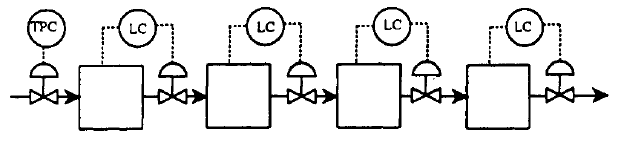
\includegraphics[width=\linewidth]{chapters/4-operation-control/4-Figures/TPM-Price-1994.png}
    \caption{Example of inventory control in direction of flow, taken from \textcite{}}
    \label{fig:TPM}
\end{wrapfigure}
Inventory control is important to maintain a steady operation of the plant with no accumulation of material in any process unit. Effective inventory controllers are those that are on the primary path, and thus exclude recycle streams. Since the TPM was at the feed to the process, all inventory controls were placed in the direction of flow in order to ensure changes to the production rate from the TPM are propagated throughout the process (see Figure \ref{fig:TPM}). 

Purge streams were added in every recycle loop to prevent the buildup of non-reactive components in process streams.  



\subsection{Challenges to control}%Marie

\subsubsection{Difficult measurements and dynamics} %0.75 page
During the plant-wide control survey, difficult measurements were identified and solutions were proposed to overcome the control challenges. Firstly, composition analysis is essential to ensure the final products met their quality specification. However composition analysis is a rather long measurement which means that there can be a long time delay between the apparition of a problem, its identification by the composition transmitter and its resolution via the control loops in place. Where possible inferential control can be implemented to reduce the time delay. For instance, the top and bottom composition of distillation column outlet streams can be controlled with temperature []. However for inferential control to be effective, robust calibration curves between the measured variable and the controlled variable must exist. Moreover the presence of impurities can significantly impact the correlation between the two process variables, ultimately leading to off-specification products. It is recommended to perform thorough experiments to obtain adequate calibration curves to be used in inferential control. In addition to inferential control with temperature, the composition can be inferred from density and viscosity measurements []. Multiplying the number of proxi measured variable should increase the accuracy of the inferential control of composition.

Furthermore, the robust control of temperature in the reactors is one of Nitroma's major concerns since all reactions are highly exothermic and could lead to thermal runaways. More specifically, in the nitration reactor R101, a hot spot can form at the centre of the catalyst bed in the shell-and-tube heat exchanger reactor, which means it can not be directly measured with temperature transmitters placed at the walls. It is suggested to conduct experiments and modelling work to develop correlations between the reactor wall temperature and the inner temperature. Additionally, the monitoring of cooling water outlet temperature can infer of the presence of a significant increase in temperature in the reactor.

Difficult dynamics can also be encountered while conducting a plant-wide control structure. Since Nitroma's process is continuous, it is expected that less difficult control dynamics will be found as opposed to a batch process. Nonetheless, it is necessary to have dynamic modelling of plant to be able to design better control loops and transfer functions.


\subsubsection{Process bottleneck} % 0.25 page

The nitration reactor R101 is Nitroma's process bottleneck since it produces the precursors for all three products made. As the first major unit in the process, any issue encountered in its operation could cascade through the whole plant. The operation conditions of this reactor indeed determine the proportions of the three products, as well as the final quantity and purity which can be obtained. 	Safety functions were installed to closely monitor and control operational parameters (temperature, pressure, flow and composition). To avoid the propagation of quality disturbances to downstream units, additional buffer tanks are installed. In addition to regular maintenance and inspection of the equipment for fouling and early catalyst deactivation, a back-up cooling system is implemented to reduce as much as reasonably feasible the risk of thermal runaway.


\subsection{Key disturbances} % 0.75 page

\subsubsection{Feed quality}
The quality of the toluene, nitric acid, formic acid, hydrogen air and methanol used in the process can significantly affect the good operation of the system. In addition to lowering the final product quality, impurities present in the feeds can decrease catalyst activity in the reactors, thus resulting in lower production and off-specification products. Mitigating strategies include the installation of feed composition analysers and a procedure to ensure storage tanks are correctly sealed. It is also recommended to use air scrubbers to purify the air used for the oxidation of PNT.

\subsubsection{Flowrate}
Variations of flowrate is one of the most prevalent disturbance in the process. Not only can it affect the overall throughput and quality, uncontrolled changes in flowrate can pose serious safety issues. A significant drop in cooling water flowrate could indeed result in a thermal runaway if the exothermic reactions can not be managed adequately. The feedforward control loops installed in the plant aim at helping the system to proactively adjust to flowrate disturbances detected upstream. The installation of back-up auxiliary equipment, such as back-up pumps, also contributes to the plant's ability to withstand flowrate disturbances.


\subsubsection{Ambient temperature}

The ambient temperature can affect the plant operation in multiple ways. Firstly, it can impact the temperature of the cooling water used to control the temperature of the reactors where exothermic reactions take place. Ineffective control could lead to thermal runaway. Moreover, air plays the role of oxidiser in the partial and complete oxidation of PNT (reactors R301 and R401). A significant change in temperature could disturb the process, having both quality and safety consequences. Finally some streams are cooled in an air heat exchanger, such as the cooler in the Rankine cycle around the PNT crystalliser. If the ambient temperature is so high that it is unable to cool down the required streams, the purity of the final products will be affected. To limit the impact of variations of the ambient air temperature on the process, it is essential to install ambient temperature transmitters on the plant and to connect them with feedfoward control loops for major units. As several units depend on tight temperature control (exothermic reactors, crystallisers), it is recommended to plan for the switch of cooling medium, for instance using a refrigerant. This would require the installation of a back-up Rankine cycle for the cooling system Another suggestion is the construction of cooling towers to provide sufficiently cold cooling water when the normal cooling water supplier fails to deliver the requirements.

\subsubsection{Utilities}

The main disturbances in key utilities include the supply of electricity and the temperature and flowrate of cooling water and steam. The fluctuations in the later have already been discussed in previous section and can be mitigated via feedforward control.
Electricity is not only key to supplying heat to process fluids through electric heaters and to running the pumps and fans, it is also essential for the actuation of electrical control valves for flow are pressure. If power is lost, back-up battery packs provide the energy required to bring the equipment and control valves to a fail-safe state, thus preventing accidents. Restarting the plant upon electrical power restoration must be correctly managed to prevent the automatic restart of some equipment before other sections are ready for operation. The installation of a robust interlock system accompanied with back-up power supplies can accommodate with temporary losses of power. However in prevision of longer outages, procedures to bring the plant to a safe state must be implemented.


\subsection{Key areas of maintenance} %0.25 page

One of the operation during plant maintenance is to remedy to catalyst deactivation. The four reactions involved in Nitroma's process indeed use solid catalysts whose catalytic activity can be weakened by impurities. Catalysts can be regenerated during planed shutdown to ensure optimum process performance. Another major operation taking place during maintenance is the inspection of electrical appliances, in particular control instruments and electric heaters. The transmitters and their associated control loops and alarms are calibrated and tested. In addition, the heating elements are inspected to assess their level of wear and tear. Finally fouling can cause major issues in mechanical integrity of the equipment. Fouling is particularly preoccupying for the crystallisers as solids could accumulate causing damage to the equipment. Fouling prevention involves regular inspection of the equipment using ultrasounds and regular cleaning.